\chapter{Ergebnisse}
\label{sec:ergebnisse}
In diesem Kapitel werden zu Beginn
die im Abschnitt  \ref{sec:floquetheo} vorgestellten
Eigenschaften der Floquet Theorie am Modell überprüft.
Des Weiteren wird die zeitliche Entwicklung
eines Zustandes, welcher durch den
Floquet Formalismus berechnet wird, mit der einer
numerischen Lösung der Schrödingergleichung verglichen.
Es wird eine Methode vorgestellt, mit der es in der
Floquet Theorie möglich ist, einen zeitlich gemittelten Strom zu berechnen.
Diese wird durch das Heranziehen des
auf konventionelle Art berechneten zeitlich gemittelten Strom überprüft.
Anschließend wird der berechnete Strom auf in dem Abschnitt
\ref{sec:inverfaraday} prognostizierten Abhängigkeiten untersucht.
Abschließend wird das Zwei-Elektronen-System betrachtet und
ebenfalls ein gemittelter Strom berechnet.

In den folgenden Rechnungen wird der Koeffizient des Tight-Binding
Hamiltonian $J$ auf $1\si{\electronvolt}$ gesetzt und
für den Gitterabstand wird ein typischer Wert von $d=\SI{4}{\angstrom}$ gewählt.
Alle anderen Größen werden im Folgenden in Einheiten von $J$ und $d$ angegeben.
Die Bandlücke $2a$ liegt in der
Größenordnung des Sprungtermes $J$ und wird
daher auf $2\,J$ gesetzt.
Die Parameter des elektrischen Feldes werden
im Bezug auf das in \cite{jackl} beschriebene Experiment gewählt.
Die Amplitude des elektrischen Feldes liegt somit um den Wert \cite{phillip}
\begin{align}
  E_0\approx\SI{69,2}{\mega\volt\per\meter}\approx\num{0,03}\, \frac{J}{d\symup{e}}.
\end{align}
Eine Frequenz des Lichtfeldes mit
einer typischen Wellenlänge $\lambda\approx\SI{800}{\nano\meter}$ ist
\begin{align}
  \omega\approx\SI{2,35}{\peta\hertz}\approx\num{1,5}\,\frac{J}{\hbar}.
\end{align}
Des Weiteren wird eine Pulsdauer
\begin{align}
 \Gamma=\SI{50}{\femto\second}\approx76\,\frac{\hbar}{J}
\end{align}
für das Lichtfeld eingeführt, in der das System beobachtet wird.
Eigenwerte und Eigenvektoren einer Matrix werden im Folgenden mit der Funktion
\textit{eig} aus dem Programm Octave \cite{octave}
berechnet. Numerische Lösungen von der Schrödingergleichung werden
durch den adaptiven Algorithmus $\textit{lsode}$ aus dem Programm octave \cite{octave} bestimmt.
Zur Überprüfung der Abhängigkeiten werden verschiedene Funktion an
die berechneten Werte angepasst, dies geschiet durch die Funktion \textit{curve-fit} von scipy \cite{scipy}.
Wichtige Naturkonstanten werden \cite{schwabl} entnommen.



\section{Frequenzabhängigkeit der Quasieigenenergien}
\label{sec:w_abb}
Zunächst werden die Eigenschaften der Floquet Theorie,
teils unabhängig von typischen Größen des Systems, untersucht. Dafür
werden die Eigenwerte
 $\epsilon_{\alpha n}$ für eine
Matrix $\mathcal{H}_\mathrm{F}$ mit Trunkierparameter $N=1$,  konstanter lokaler Energie $a=1\,J$
und elektrischer Feldamplitude $E_0=1\,\frac{J}{d\symup{e}}$
für Frequenzen in einem Bereich von $\omega\in\left[0,6\right]\,\frac{J}{\hbar}$ berechnet.
Um die Effekte des periodischen Potentials
$V(t)$ zu verdeutlichen,
werden ebenfalls Eigenwerte $E_{\alpha n}$ für eine Matrix
$\mathcal{H}_F$ mit $E_0=0\,\frac{J}{d\symup{e}}$, dies beschreibt den
zeitunabhängigen Fall, berechnet, sodass in Abbildung \ref{fig:epsilon_f}
die berechneten Eigenwerte verglichen werden können.
\begin{figure}
   \centering
   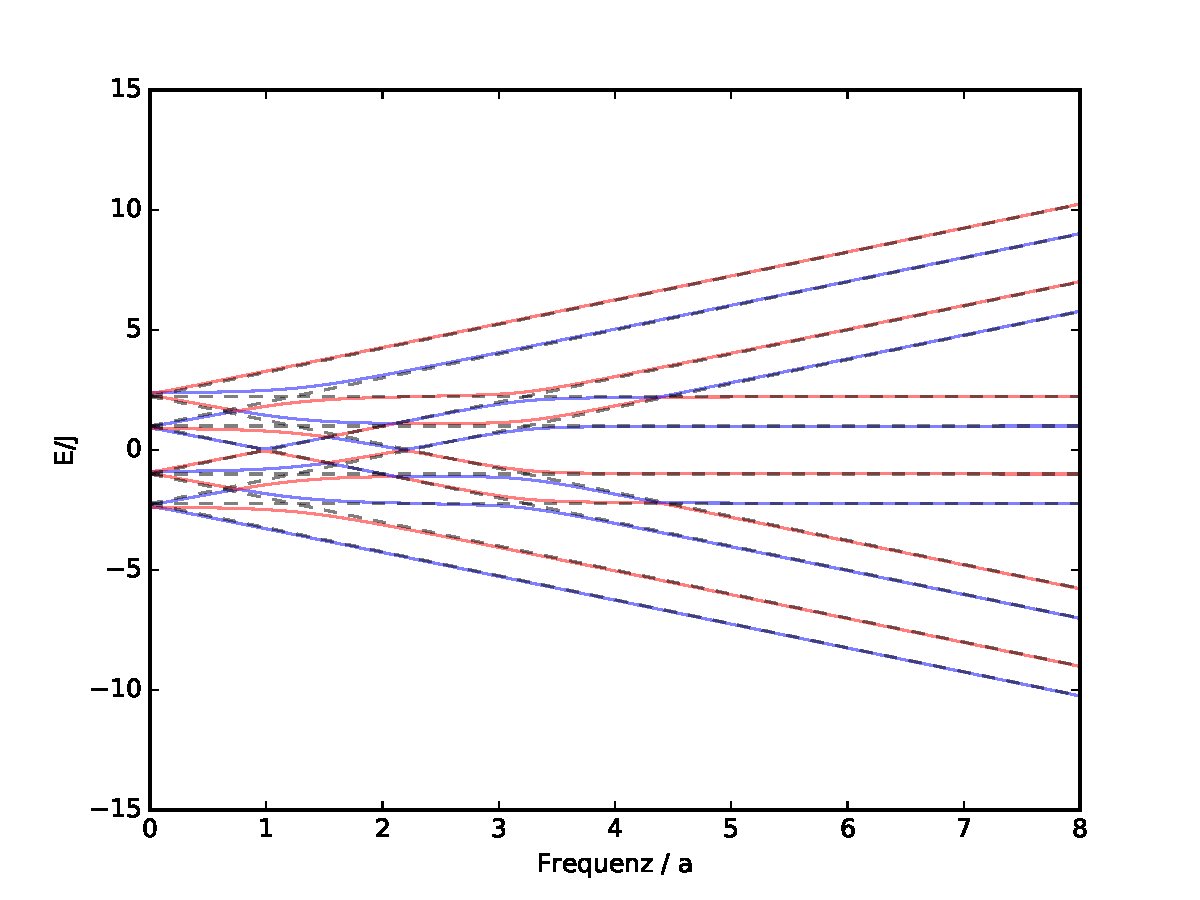
\includegraphics[width=0.7\textwidth]{Programme/Freqenzen_kontinuierlich/Plots/Plot_fur_a=1.0_E=1.0.pdf}
   \caption{Eigenwerte $\epsilon_{\alpha n}$ der Matrix $\mathcal{H}_\mathrm{F}$
    für $a=1\,J$ und $E_0=1\,\frac{J}{d\symup{e}}$ und
   Eigenwerte $E_{\alpha n}$ von $\mathcal{H}_\mathrm{F}$ für das
   zeitunabhängigen Systems $E_0=0\,\frac{J}{d\symup{e}}$
  für einem Trunkierparameter $N=1$ in Abhängigkeit von der Frequnez $\omega$.}
   \label{fig:epsilon_f}
\end{figure}
In der Abbildung \ref{fig:epsilon_f} können, wie in \cite{haenggi} beschrieben,
an Stellen, wo es zur
Überschneidung der Eigenwerte  $E_{\alpha n}$
des zeitunabhängigen Systems kommt, die Phänomene des "avoided crossing" und
"exact crossing" der QEE $\epsilon_{\alpha n}$ beobachtet werden,
die durch das zeitabhängige elektrische Feld hervorgerufen werden.
%??vielleicht??


\section{Brillouin-Zone der Quasieigenenergien}
\label{sec:E_abb}
In diesem Abschitt wird die Darstellbarkeit der QEE, wie in
Abschitt \ref{sec:floquetheo}
beschrieben, in der 1.
Brillouin-Zone untersucht.
Dafür werden QEE bei einer konstanten Frequenz $\omega=1\,\frac{J}{\hbar}$ und
lokaler Energie $a=1\,J$ in Abhängigkeit von der
Amplitude $E_0$, die hier zur Veranschaulichung im
Bereich $E_0\in\left[0,5\right]\,\frac{J}{d\symup{e}}$ liegt, berechnet.
Diese sind in der Abbildung \ref{fig:brillouin} gegen $E_0$ aufgetragen.
Zusätzlich wird der Trunkierparameter $N\in\{1,3,5,6\}$ der Matrix $\mathcal{H}_F$ variiert.
%
% \begin{figure}
%   \centering
%   \begin{subfigure}{0.48\textwidth}
%     \includegraphics[width=1\textwidth]{Programme/Energien_kontinuierlich/Plots/Plot_fur_a=1.0_w=1.0N=1.0.pdf}
%     \caption{Trunkierparameter $N=1$.}
%     \label{fig=N_1}
%   \end{subfigure}
%   \begin{subfigure}{0.48\textwidth}
%     \includegraphics[width=1\textwidth]{Programme/Energien_kontinuierlich/Plots/Plot_fur_a=1.0_w=1.0N=3.0.pdf}
%     \caption{Trunkierparameter $N=3.$}
%     \label{fig=N_3}
%   \end{subfigure}
%   \begin{subfigure}{0.48\textwidth}
%     \includegraphics[width=1\textwidth]{Programme/Energien_kontinuierlich/Plots/Plot_fur_a=1.0_w=1.0N=5.0.pdf}
%     \caption{Trunkierparameter $N=5$.}
%     \label{fig=N_5}
%   \end{subfigure}
%   \begin{subfigure}{0.48\textwidth}
%     \includegraphics[width=1\textwidth]{Programme/Energien_kontinuierlich/Plots/Plot_fur_a=1.0_w=1.0N=6.0.pdf}
%     \caption{Trunkierparameter $N=6$.}
%     \label{fig=N_6}
%   \end{subfigure}
%   \caption{Berechnete $\epsilon_{\alpha n}$ für unterschiedliche
%   Trunkierparameter $N\in\{1,3,5,6\}$
%   der Matrix $\mathcal{H}_F$ in Abhängigkeit von der Ampiltude $E_0$
%   bei einer lokalen Energie $a=1\,J$ und einer Frequenz
%   $\omega=1\,\frac{J}{\hbar}$. Die gestrichelten Linien grenzen dabei
%   die verschiedenen Brillouin-Zonen ab.}
%   \label{fig:brillouin}
% \end{figure}

Es wird deutlich, dass für kleine Trunkierparameter $N$ die Bedingung
für eine Darstellung in der 1. Brillouin-Zone nicht erfüllt ist.
Zudem wird beobachtet, dass die Übereinstimmung
der 2. Brillouin-Zone mit der 1. Brillouin-Zone mit
größeren Parameter $N$ zunimmt.
Weiterhin zeigt sich eine Abhängigkeit zu der Ampiltude $E_0$, da
größere Ampiltuden ebenfalls ein größerer Trunkierparameter $N$
benötigt wird, um die korrekten QEE zu berechnen.
Diese Beobachtungen zeigen, dass es möglich ist, die
QEE $\epsilon_\alpha$  für ein ausreichend großen Trunkierparameter
 $N$ in die erste Brillouin-Zone
mit $\epsilon_\alpha \in\left[-\frac{\omega}{2},\frac{\omega}{2}\right]$
 darzustellen.
Alle anderen QEE $\epsilon_{\alpha n}$ lassen sich somit
durch die Periodizitätsbedingung \eqref{eqn:epsilon_n} berechnen.
In der ersten Brillouin-Zone, siehe Abbildung \ref{fig:brillouin},
existieren genau vier QEE, folglich besitzt das System
vier QEE und vier QEZ.
Aus der Abbildung \ref{fig:brillouin} wird entnommen, dass
für Rechnungen mit einer Amplitude $E_0<1\,\frac{J}{d\symup{e}}$ ein
Trunkierparamter $N=3$ genügt, um die korrekten QEE zu berechnen.
%Aus der  Abbildung \ref{fig:brillouin} kann entnommen werden, System vier Quasienergien besitzt

\section{Orthogonalität der Quasieigenzustände}
\label{sec:ortho}
Im Folgenden wird die Orthogonalität zwischen den
QEZ $\ket{\Phi_\alpha}$ aus der Gleichung
\eqref{eqn:ortho} für
unterschiedliche Trunkierparameter $N$ der Matrix $\mathcal{H}_F$ überprüft.
Dafür wird $\braket{\phi_\beta\vert\phi_\alpha}$
in Abhängigkeit von dem Parameter $N$
für die Werte    $a=1\, J$, $E_0=\num{0,03}\,\frac{J}{d\symup{e}}$  und $\omega=1\,\frac{J}{\hbar}$ untersucht.
In der Abbildung \ref{fig:ortho} wird nur $\beta=1$ dargestellt, da $\beta\in\{2,3,4\}$ identische Ergebnisse liefert.

\begin{figure}
    \centering     % vielleicht mit 2x2 subfigure
    \includegraphics[width=0.7\textwidth]{Programme/Orthogonalitat_der_quasizustande/Plots/Potential=1.0/Energie=0.03/Frequenz=1.0/Plot_fur_phi1_phi_i}
    \caption{Das Skalarprodukt $\braket{\Phi_1|\Phi_\alpha}$ in Abhängigkeit von dem Trunkierparameter $N$ der Matrix $\mathcal{H}_F$ für
    $a=1\, J$ , $E_0=0,03\,\frac{J}{d\symup{e}}$  und $\omega=1\,\frac{J}{\hbar}$. }
     \label{fig:ortho}
\end{figure}
Aus Abbildung \ref{fig:ortho} wird entnommen, dass bei geringem Parameter $N$ die Orthogonalität der QEZ
nicht gegeben ist.
Für die in Abbildung \ref{fig:ortho} verwendeten Größen
erweist sich der Wert $N=3$ als ausreichend zur Gewährleistung der Orthogonalität.
Es stellt sich weiterhin ein antiproportionaler Zusammenhang von lokaler Energie
$a$ und Frequenz $\omega$ zu dem
benötigten Parameter $N$ heraus.
Wegen der Antiproportionalität ist es notwendig,
bei den folgenden Berechnungen für
Werte von $\omega<1\,\frac{J}{\hbar}$ und $a<1\,J$ die
Orthogonalität der QEZ zu überprüfen.
Andernfalls reicht eine Matrixgröße
von $N=3$ zum Erfüllen der Orthogonalitätsbedingung aus.



% -über formel .. kann quasizustand berechnet werden
% -die Orthogonalitäts bedingung formel .. sollte erfüllt sein

\section{Zeitentwicklung eines Zustandes durch den Floquet Formalismus}
\label{sec:zeit}
In diesem Abschnitt wird eine Zeitentwicklung des zeitabhänigigen
Ein-Elektron-Systems
durch den Floquet Formalismus bestimmt.
Als Startzustand $\ket{\Psi_0}$ wird der Grundzustand $\ket{\phi_1}$ des zeitunabhängigen Systems verwendet, da
das System zu Beginn im Zustand niedrigster Energie verweilt.
Es wird die Zeitentwicklung für eine Frequenz $\omega$ des elektrischen Feldes
abseits von Resonanzfrequenzen, welche für ein System mit $a=1\,J$ in
Tabelle \ref{tab:w_res} aufgelistet sind,
betrachtet.
\begin{table}
  \centering
  \caption{Resonanzfrequenzen $\omega_{\text{res}_i}$ in einem System mit $a=1 J$,
   welche sich aus der Gleichung \eqref{eqn:Resonanz} ergeben.}
  \label{tab:w_res}
\begin{tabular}{c | c c c}
\toprule
$a/\,J$ & $\omega_{\text{res}_1}/ \frac{J}{\hbar}$ & $\omega_{\text{res}_2}/\frac{J}{\hbar}$ & $\omega_{\text{res}_3}/\frac{J}{\hbar}$ \\
\midrule
\num{1}  &  \num{1,24}  & \num{3,24} &  \num{4,47}  \\
\bottomrule
\end{tabular}
\end{table}

% -oder -
%
% In der Abbildung \ref{fig:Resonanz} sind
% die Resonanzfrequenzen \eqref{eqn:Resonanz} in Abhängigkeit
% von den lokalen Energien aufgetragen.
%
% \begin{figure}
%   \centering
%   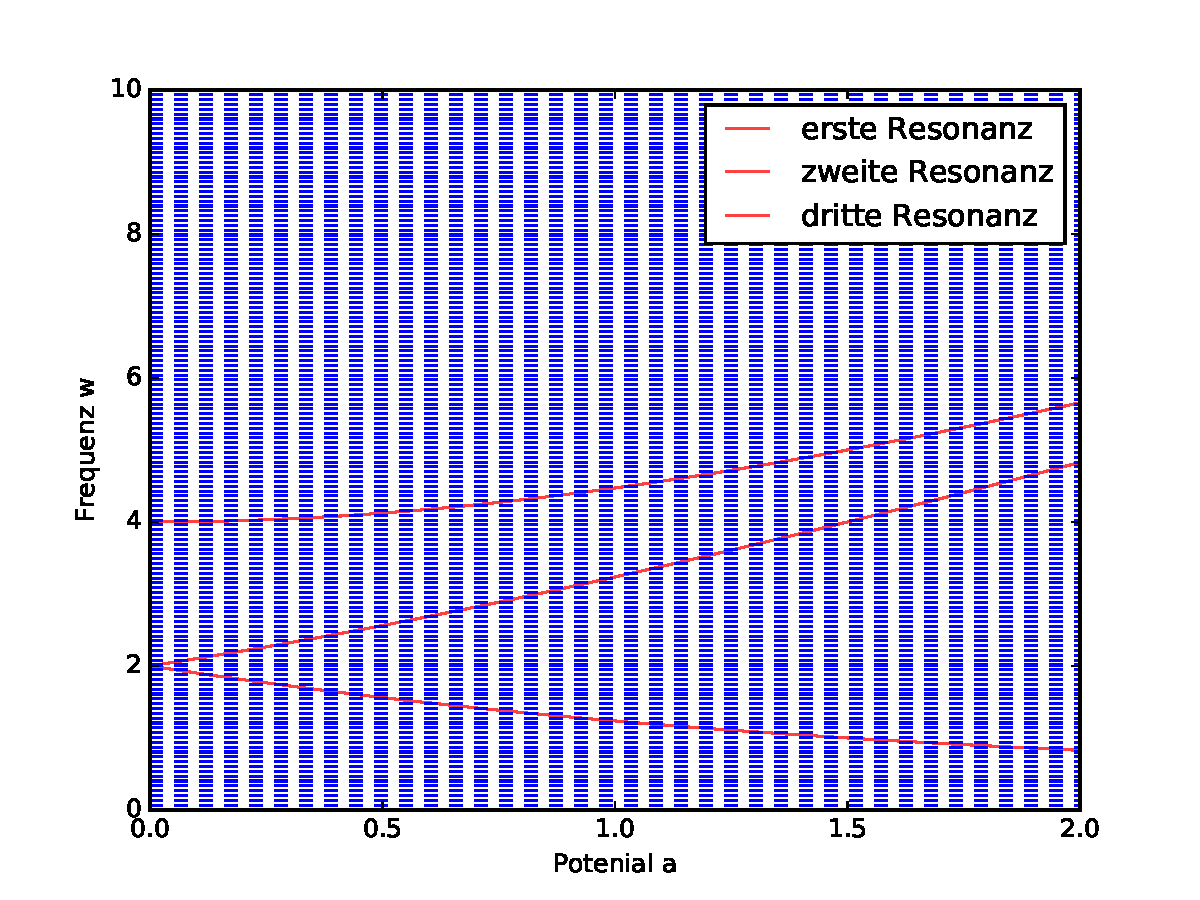
\includegraphics[width=0.7\textwidth]{Programme/Eigenzustande/Plots/Resonanzen.pdf}
%   \caption{Resonanzfrequenzen in Abhängigkeit von der lokalen Energie $a$}
%   \label{fig:Resonanz}
% \end{figure}


Unter dem Ausschluss der Resonanzfrequenzen aus der
Tabelle \ref{tab:w_res},
  % /Abbildung \ref{fig:Resonanz},
wird bei einer lokalen Energie von
$a=\num{1}\, J$ und einer Amplitude von $E_0=\num{0,03}\,\frac{J}{d\symup{e}}$
die Frequenz $\omega=\num{1,5}\,\frac{J}{\hbar}$ gewählt.
Für diese Werte wurde
in den Abschnitten \ref{sec:E_abb} und \ref{sec:ortho} gezeigt, dass ein
Trunkierparameter von $N=3$ ausreicht, um die QEE und QEZ
korrekt zu berechnen.
Um die Zeitentwicklung nach Floquet durchführen zu können, wird
zunächst durch die Gleichung \eqref{eqn:super} der Grundzustand
als Superposition der QEZ ausgedrückt.
Durch Anwenden des Zeitpropagators \eqref{eqn:Propagator} auf den Grundzustand
ist es möglich, den zeitentwickelten Grundzustand
$\ket{\Psi(t)}$ zu berechnen.
In Abbildung \ref{fig:zeitentwicklung} ist
die Aufenthaltswahrscheinlichkeit
$P_i(t)=\lvert\braket{i|\Psi(t)}\rvert^2$ für
die vier unterschiedlichen Gitterplätze in Abhängigkeit von der Zeit dargestellt.
Dabei wird ebenfalls die Aufenthaltswahrscheinlichkeit $P_{i_\text{num}}(t)$
einer numerischen Lösung
der Schrödingergleichung für den Grundzustand aufgetragen.
% durch den
% adaptiven Algorithmus $\textit{lsode}$,
% ??der durch das Programm Octave \cite{octave} bereitgestellt wird,?? aufgetragen.

\begin{figure}
  \centering
  \includegraphics[width=0.7\textwidth]{Programme/Eigenzustande/Plots/Potential=1.0/Energie=0.03/Besetzungen(t)_mit_Floquet_N=3w=1.5.pdf}
  \caption{Aufenthaltswahrscheinlichkeit des zeitentwickelten Grundzustandes für den $i$-ten Gitterplatz
  sowohl von dem Floquet Formalismus $P_i$ als auch von
  einer numerische Lösung $P_{i_\text{num}}$
  in Abhängigkeit von der Zeit $t$ für
  $a=1\,J$, $\omega=\num{1,5}\,\frac{J}{\hbar}$ und  $E_0=\num{0,03}\,\frac{J}{d\symup{e}}$.
  Die gestrichelten Linien markieren dabei die Periodendauer $T$ des elektrischen Feldes und
  der schwarze Balken die zu Beginn erwähnte Pulsdauer $\Gamma$ des Licht-Feldes.}
  \label{fig:zeitentwicklung}
\end{figure}

Es zeigt sich, dass die verschiedenen Lösungswege dieselben Ergebnisse liefern.
Somit ist die Richtigkeit der Zeitentwicklung in der Floquet Theorie bestätigt.
Außerdem ist erkennbar, dass die Gitterplätze $1$ und $3$
bevorzugt sind. Dies ist durch die Struktur des Bandisolators begründet. Die beiden Position besitzen
eine geringere lokale Energie $a$ als die anderen beiden Plätze.
%
% -wenn Zustände orthogonal zeitentwicklung möglich
% -vergleich mit lsode
% -stimmt überein eignet sich folglich für zeitentwicklung

\section{Untersuchung des Stromes in einem Bandisolator}
Die in Abschnitt \ref{sec:zeit} bestätigte Zeitentwicklung eines Zustandes durch den Floquet Formalismus
wird in diesem Abschnitt zur Berechnung des Stromflusses im System, welches sich zu Beginn im Grundzustand befindet,  genutzt.
Der Erwartungswert des Stromflusses im System ergibt sich aus dem Erwartungswert
\begin{align}
\braket{I}(t)=\braket{\psi(t)\lvert I \rvert\psi(t)}
\intertext{des Stromdichteoperators\cite{schwabl}}
I= \symup{i}\frac{J}{4}\sum_i^4 \left(c_{i+1}^\dag c_{i}^{\phantom{\dag}}  -c_{i}^\dag c_{i+1}^{\phantom{\dag}}\right).
\end{align}
Es werden wieder die Einheitsvektoren $\vec{e}_i$ als Basis gewählt, sodass
sich die Matrixdarstellung des Stromdichteoperators
\begin{align}
I=\symup{i}\frac{J}{4}\begin{pmatrix}
  \phantom{-}0&           -1 &\phantom{-}0 & \phantom{-}1 \\
  \phantom{-}1& \phantom{-}0 &          -1 & \phantom{-}0\\
  \phantom{-}0& \phantom{-}1 &\phantom{-}0 &           -1 \\
            -1& \phantom{-}0 &\phantom{-}1 & \phantom{-}0
\end{pmatrix}
\end{align}
ergibt.
Die Abbildung \ref{fig:strom_t} enthält den Erwartungswert des Stromflusses $\braket{I}(t)$ in Abhängigkeit von der Zeit.
\begin{figure}
  \centering
  \includegraphics[width=0.7\textwidth]{Programme/Strom/Plots/Potential=1.0/Energie=0.03/Stromerwartungswert(t)_N=3w=1.5.pdf}
  \caption{Erwartungswert des Stromflusses $\braket{I}(t)$ im System in Abhängigkeit der Zeit $t$ für
  $a=1\,J$, $\omega=\num{1,5}\,\frac{J}{\hbar}$ und  $E_0=\num{0,03}\,\frac{J}{d\symup{e}}$.
  Die gestrichelten Linien markieren dabei die Periodendauer $T$ des elektrischen Feldes und
  der schwarze Balken markiert die zu Beginn erwähnte Pulsdauer $\Gamma$ des Licht-Feldes.}
 \label{fig:strom_t}
\end{figure}

Da für den IFE , wie in dem Abschnitt
\ref{sec:inverfaraday} beschrieben, nur ein in der Zeit gemittelter
Stromfluss zur Magnetisierung $M$ beiträgt, wird hier der
Erwartungswert $\braket{I}$ des Stromflusses über eine Zeitspanne $T$
gemittelt. Der zeitlich
gemittelte Erwartungswert des Stromflusses $\bar{\braket{I}}$ ergibt sich aus
\begin{align}
  \bar{\braket{I}}= \frac{1}{T}\int_0^{T} \braket{\Psi(t)|I|\Psi(t)}. \label{eqn:mittelwert}
\end{align}
%Mit Hilfe des Zeitpropagators \eqref{eqn:Propagator}
In dem Floquet Formalismus ist es möglich, zeitlich
gemittelte Erwartungswerte von
Operatoren wie dem Stromdichteoperator zu berechnen.\cite{haenggi}
Durch Einsetzen von \eqref{eqn:psi_t} und \eqref{eqn:fourier}
in die Gleichung \eqref{eqn:mittelwert} ergibt sich nach Ausführung der Integration
 \begin{align}
 \bar{\braket{I}}&= \lim_{N\to\infty}\sum_\alpha \lvert c_\alpha \rvert^2  \sum_{-N}^{N} \braket{c_\alpha^n\lvert I \rvert c_\alpha^n}  \label{eqn:mittel}
 \intertext{mit}
  c_\alpha&=\braket{\Psi_0\vert\Phi_\alpha}.
\end{align}
In dem Floquet Formalismus ist es somit nicht
notwendig, erst den Erwartungswert $\braket{I}(t)$
zu bestimmen und den Mittelwert über die Gleichung \eqref{eqn:mittelwert}
zu berechnen. Die Formel \eqref{eqn:mittel} ermöglicht es, den
zeitlich gemittelte Erwartungswert $\bar{\braket{I}}$ direkt zu berechnen.
Zur Überprüfung von Gleichung \eqref{eqn:mittel} wird
der zeitlich gemittelte Stromerwartungswert $\bar{\braket{I}}$
für unterschiedliche Frequenzen
$\omega\in\{\num{1,0},\num{1,5},\num{2}\}\,\frac{J}{\hbar}$
in Abhängigkeit von der Amplitude
des elektrischen Feldes
$E_0\in\left[\num{0},\num{0,1}\right]\,\frac{J}{d\symup{e}}$ auf
zwei verschiedene Methoden berechnet.
Zum einen wird die Gleichung \ref{eqn:mittel}, welche die Floquet Theorie
bereitstellt, verwendet $\bar{\braket{I}}_F$ und zum anderen wird der berechnete Stromerwartungswert
über eine
Zeitspanne $T$, hier die Pulslänge $\Gamma$ des Lichtfeldes,
gemittelt $\bar{\braket{I}}_M$ .
Die Abbildung \ref{fig:E_Strom} enthält jeweils die aus
den zwei verschiedenen Methoden für $a=1\,J$
berechneten zeitlich gemittelten Ströme $\bar{\braket{I}}$.

\begin{figure}
  \centering
  \includegraphics[width=0.7\textwidth]{Programme/Strom_mittelwerte/Plots_mittelwerte/Potential=1.0Stromerwartungswert(t)_N=3.pdf}
  \caption{Zeitlicher Mittelwert des Stromerwartungswerts $\bar{\braket{I}}$,
    welcher durch zweite Methoden
  für $a=1\,J$ und
  unterschiedliche Frequenzen
  $\omega\in\{\num{1,0},\num{1,5},\num{2}\}\,\frac{J}{\hbar}$
  in Abhängigkeit von der Amplitude elektrischen Feldes $E_0$ berechnet wird. }
  \label{fig:E_Strom}
\end{figure}

Aus Abbildung \ref{fig:E_Strom} tritt hervor,
dass die Gleichung \eqref{eqn:mittel} identische
Ergebnisse wie die Mittelung über eine Zeitspanne liefert.
Geringe Abweichungen sind dadurch erklärbar, dass
die Methode der Floquet Theorie den zeitlichen gemittelten Stromerwartungswert
des eingeschwungen Systems beschreibt, wohingegen die
Mittelung über die Pulslänge $\Gamma$ Einschwingungsvorgänge des Systems
mit berücksichigt.
Auf diese Weise ist bestätigt, dass der zeitlich gemittelte
Stromerwartungswert $\bar{\braket{I}}$
über die Gleichung \eqref{eqn:mittel}
berechnet werden kann.
Im Folgenden wird daher die Methode, welche die Floquet Theorie bereitstellt,
um zeitlich gemittelte Stromerwartungswerte zu berechnen,
verwendet.

\section{Überprüfung der Stromabhängigkeiten in einem Bandisolator}
\label{sec:abbhangig}
Wie in dem Kapitel \ref{sec:inverfaraday} beschrieben,
soll der Strom bei dem IFE
in einem Isolator quadratisch
mit der Amplitude des elektrischen Feldes $E_0$
sowie linear mit der Frequenz $\omega$ des elektrischen
Feldes steigen. Diese Abhängigkeiten werden in diesem Abschnitt für das
Ein-Elektron-System überprüft.
Für die quadratische Abhängigkeit wird in der Abbildung
\ref{fig:E_abb} der zeitliche gemittlte Strommerwartungswert $\bar{\braket{I}}$
 gegen $E_0$ aufgetragen.
Wieder werden die Frequenzen
$\omega\in\{\num{1},\num{1,5},\num{2}\}\,\frac{J}{\hbar}$
 bei einer lokalen Energie von $a=1\,J$ verwendet.
An die berechneten Werte wird versucht, eine quadratische Funktion $f(x)=ax^2$
zu fitten, ebenfalls
in Abbildung \ref{fig:E_abb} zu sehen.

\begin{figure}
  \centering
  \includegraphics[width=0.7\textwidth]{Programme/Strom_fit_e/Plots_mittelwerte/Potential=1.0Stromerwartungswert(t)_N=3.pdf}
  \caption{Der zeitlich gemittelte Stromerwartungswert $\bar{\braket{I}}$  für $a=1\,J$ und
  unterschiedliche Frequenzen $\omega\in\{\num{1,0},\num{1,5},\num{2}\}\,\frac{J}{\hbar}$
  und entsprechende Fit-Funktion in Abhängikeit von der Amplitude des elektrischen Feldes $E_0$. }
  \label{fig:E_abb}
\end{figure}

Die Abbildung \ref{fig:E_abb} bestätigt, dass es
möglich ist, eine quadratische Funktion an die berechneten Werte zu fitten.
Folglich ist die quadratische Abhängigkeit zu der Amplitude des elektrischen Feldes $E_0$
bestätigt.
Abschließend gilt es, die Linearität des zeitlich gemittelten
Stromerwartungswertes
zur Frequenz zu untersuchen.
Hierfür wird der zeitlich gemittelte
Stromerwartungswert $\bar{\braket{I}}$
in Abhängigkeit von der Frequenz $\omega$ in einem
Bereich $\omega\in \left[0,8\right]\,\frac{J}{\hbar}$ für
zwei verschiedene elektrische Amplituden
$E_0\in\{\num{0,01},\num{0,03},\num{0,05}\}\,\frac{J}{d\symup{e}}$
untersucht, siehe Abbildung \ref{fig:w_abb}.
Es wird eine lokale Energie von $a=1\,J$ verwendet.

\begin{figure}
   \centering
   \includegraphics[width=0.7\textwidth]{Programme/Strom_frequenzabb/Plots_mittelwerte/Potential=1.0Stromerwartungswert(t)_N=3.pdf}
   \caption{Der zeitlich gemittelte Stromerwartungswert $\bar{\braket{I}}$
  für $a=1J$, unterschiedliche Amplituden
   $E_0\in\{\num{0,01},\num{0,03},\num{0,05}\}\frac{J}{d\symup{e}}$
   in Abhängigkeit von der Frequenz des Lichtfeldes $\omega$.}
   \label{fig:w_abb}
\end{figure}

In Abbildung \ref{fig:w_abb} werden Resonanzeffekte
bei den zuvor berechneten Resonanzfrequenzen $\omega_{\text{res}_i}$
beobachtet. Auf Grund der
dominierenden Resonanzeffekte in Abbildung \ref{fig:w_abb}
lässt sich die Linearität nicht eindeutig bestätigen.
Um die Resonanzeffekte nicht zu betrachten, wird ein
kleinerer Frequenzbereich
$\omega\in\left[\num{0},\num{0,8}\right]\,\frac{J}{\hbar}$ untersucht.
Jedoch kommt es in diesem Bereich zu einem zunächst nicht erklärbarem
Abfall des zeitlich gemittelten Stromerwartungswertes.
Eine mögliche Ursache dafür ist eine in diesem
Frequenzbereich nicht mehr gewährleistete Orthogonalität der
QEZ, da bei einem Trunkierungsparamter von $N=3$
die Orthogonalität der QEZ nur für Frequenzen
von $\omega\geq1\,\frac{J}{\hbar}$ gewährleitet ist.
Um dies zu untersuchen, wird das Skalarprodukt der QEZ gegen
die Frequenz \omega in der Abbildung \ref{fig:N_3} für $N=3$ aufgetragen.
%Dies geschieht ebenfalls für  $N=10$, $N=20$ und $N=50$
%
% \begin{figure}
%    \centering
%    \begin{subfigure}{0.48\textwidth}
%        \includegraphics[width=1\textwidth]{Programme/Orthogonalitat_der_quasizustande_frequenz/Plots/Potential=1.0/Energie=0.028/Anzahl=3/Plot_fur_phi1_phi_i.pdf}
%        \caption{Trunkierparameter $N=3$}
%        \label{fig:N_3}
%      \end{subfigure}
%      \begin{subfigure}{0.48\textwidth}
%        \includegraphics[width=1\textwidth]{Programme/Orthogonalitat_der_quasizustande_frequenz/Plots/Potential=1.0/Energie=0.028/Anzahl=10/Plot_fur_phi1_phi_i.pdf}
%        \caption{Trunkierparameter $N=10$}
%        \label{fig:N_10}
%      \end{subfigure}
%      \begin{subfigure}{0.48\textwidth}
%        \includegraphics[width=1\textwidth]{Programme/Orthogonalitat_der_quasizustande_frequenz/Plots/Potential=1.0/Energie=0.028/Anzahl=20/Plot_fur_phi1_phi_i.pdf}
%        \caption{Trunkierparameter $N=20$}
%        \label{fig:N_20}
%      \end{subfigure}
%      \begin{subfigure}{0.48\textwidth}
%        \includegraphics[width=1\textwidth]{Programme/Orthogonalitat_der_quasizustande_frequenz/Plots/Potential=1.0/Energie=0.028/Anzahl=50/Plot_fur_phi1_phi_i.pdf}
%        \caption{Trunkierparameter $N=50$}
%        \label{fig:N_50}
%      \end{subfigure}
%      \caption{Das Skalarprodukt $\braket{\Phi_1|\Phi_\alpha}$
%       für unterschiedliche Trunkierparameter $N\in\{3,10,20,50\}$
%       der Matrix $\mathcal{H}_F$
%       in Abhängigkeit von der Frequenz $\omega$
%       für $a=1\, J$ und $E_0=\num{0,03}\,\frac{J}{d\symup{e}}$}
%     \label{fig:N_gross}
% \end{figure}


Die Abbildung \ref{fig:N_3} bestätigt
die Vermutung der fehlenden Orthogonalität.
Folglich muss der Trunkierparameter $N$ der Matrix
$\mathcal{H}_F$ erhöht werden.
Die Abbildung \ref{fig:N_gross} enthält ebenfalls
den gleichen Zusammenhang
aus \ref{fig:N_3} jedoch für
größere Parameter $N\in\{10,20,50\}$.
Es zeigt sich, dass für höhere Paramter $N$ geringere Frequenzen
erreicht werden, welche die Orthogonalitätsbedingung
erfüllen. Durch den antiproportionalen Zusammenhang
folgt, dass geringere
Frequenzen einen hohen Trunkierungsparamter $N$
benötigen. Als Folge dessen
wird die Matrix $\mathcal{H}_F$ ebenfalls
größer was sich negativ auf die Berechnungszeit
der QEE auswirkt. Deshalb ist die Floquet Matrix Methode
für geringe Frequenzen nicht günstig.
Demzufolge ist es notwendig, bei Untersuchung des linearen Bereiches eine
größere Matrix $\mathcal{H}_F$ aufzustellen. Hier soll ein Paramter von $N=50$ genügen,
folglich dürfen Frequenzen kleiner als $\num{0,1}\,\frac{J}{\hbar}??$
 bei der Überprüfung der Linearität nicht
berücksichtigt werden.
Der zeitlich gemittelte Stromerwartungswert $\bar{\braket{I}}$
wird im zuvor geforderten Frequenzbereich $\omega\in\left[0,\num{0,8}\right]\,\frac{J}{\hbar}$
gegen $\omega$ aufgetragen, siehe Abbildung \ref{fig:geraden_fit}.
Bei Frequenzen um $\num{0,65}\,\frac{J}{\hbar}$
machen sich bereits Resonanzeffekte bemerkbar,
deshalb wird versucht eine Gerade im Frequenzbereich $\omega\in\left[\num{0,1},\num{0,5}\right]\,\frac{J}{\hbar}$
an die berechneten Werte zu fitten.
\begin{figure}
    \centering
    \includegraphics[width=0.5\textwidth]{Programme/Strom_geraden_fit/Plots_mittelwerte/Potential=1.0Stromerwartungswert(t)_N=50.pdf}
    \caption{Der zeitlich gemittelte Stromerwartungswert $\bar{\braket{I}}$  für $a=1\,J$,
    unterschiedliche Amplituden des elektrischen Feldes $E_0\in\{\num{0,01},\num{0,03},\num{0,05}\,\frac{J}{d\symup{e}}$
    und entsprechende Ausgleichsgerade in Abhängikeit von der Frequenz $\omega$. }
    \label{fig:geraden_fit}
\end{figure}
Die berechneten Werte und die Ausgleichsgeraden liegen im Bereich $\omega\in\left[\num{0,1},\num{0,5}\right]\,\frac{J}{\hbar}$ übereinander.
Aufgrund dessen kann der lineare Zusammenhang
zwischen der Frequenz und dem zeitlich gemittelten Stromerwartungswert
in diesem Frequenzbereich bestätigt werden.

% -berechung des Stromes
% -überprüfung der quadratischen Ahängigkeit der Stromes
% -frequenz abhängigkeit überprüfen (gerade)
% -für kleine frequenz problem mit orthogonalität

\section{Zwei-Elektronen-System}
Um einen zeitlich gemittelten Stromerwartungswert $\bar{\braket{I}}$
in dem Zwei-Elektronen-System,
welches sich im Grundzustand befindet, zu berechnen,
wird der zeitlich gemittelten Stromerwartungswert $\bar{\braket{I}}$
für das Ein-Elektron-System
sowohl im Grundzustand als
auch im ersten angeregeten Zustand
berechnet. Aus Addition der beiden
Ein-Elektron-Ströme ergibt sich der zeitlich gemittelte Stromerwartungswert
des Zwei-Elektronen-Systems.\cite{phillip}
Die Abbildung \ref{fig:2e} enthält
den zeitlich gemittelten Stromerwartungswert $\bar{\braket{I}}$ des Zwei-Elektronen-Systems
in Abhängigkeit der Amplitude
des elektrischen Feldes $E_0$.
Wie zuvor wird das System
für die Frequenz $\omega\in\{\num{1},\num{1,5},\num{2}\}\,\frac{J}{\hbar}$
und $a=1\,J$ betrachtet.
\begin{figure}
   \centering
   \includegraphics[width=0.5\textwidth]{Programme/Zwei_elektronen/Plots_mittelwerte/Potential=1.0Stromerwartungswert(t)_N=3.pdf}
   \caption{Der zeitlich gemittelte Stromerwartungswert des Zwei-Elektronen-System $\bar{\braket{I}}$ für $a=1\,J$,
   unterschiedliche Frequenzen $\omega\in\{\num{1,0},\num{1,5},\num{2}\}\,\frac{J}{\hbar}$
   und entsprechender Fit-Funktion in Abhängikeit von der Amplitude des elektrischen Feldes $E_0$. }
   \label{fig:2e}
\end{figure}
Es zeigt sich, dass in dem Zwei-Elektronen-System keine quadratische Abhängigkeit zu der elektrischen Amplitude
vorliegt. Des Weiteren unterscheidet sich der zeitlich gemittelte Stromerwartungswert in dem Bereich
$E_0\in\left[0,\num{0,1}\right]\,\frac{J}{d\symup{e}}$ um eine Größenordnung von $10^{-5}$ von
dem im Ein-Elektron-System.
Wie in dem Abschnitt \ref{sec:abbhangig} wird ebenfalls die Frequnezabhängigkeit untersucht.
In der Abbildung \ref{fig:2_w} ist der zeitlich gemittelte Stromerwartungswert $\bar{\braket{I}}$ gegen die Frequenz $\omega$
für $E_0\in\{\num{0,01},\num{0,03},\num{0,05}\}\,\frac{J}{d\symup{e}}$ und $a=1\,J$ aufgetragen.
\begin{figure}
   \centering
   \includegraphics[width=0.5\textwidth]{Programme/Strom_zwei_El_w_abb/Plots_mittelwerte/Potential=1.0Stromerwartungswert(t)_N=3.pdf}
   \caption{Der zeitlich gemittelte Stromerwartungswert $\bar{\braket{I}}$  des Zwei-Elektronen-System
   für $a=1\,J$,
   unterschiedliche Amplituden des elektrischen Feldes $E_0\in\{\num{0,01},\num{0,03},\num{0,05}\,\frac{J}{d\symup{e}}$
  in Abhängikeit von der Frequenz $\omega$. }
   \label{fig:2_w}
\end{figure}
Aus der Abbildung \ref{fig:2_w} kann entnommen werden, dass
bei einem Zwei-Elektronen-System
fast keine Stromfluss existiert, da
selbst bei den möglichen Resonanzfrequenzen
das System keine Resonazerscheinungen aufweißt.
Eine Mögliche Ursache für das
Fehlen des Stromflusses ist das bei
zwei Elektronen das wirkende Pauliverbot den
Stromfluss einschränkt.
